\documentclass[tikz]{standalone}
\usepackage{pgfplots}

\pgfplotsset{compat=1.9}
\usepgfplotslibrary{dateplot}
\usetikzlibrary{intersections, positioning, calc, shapes}
\definecolor{color1}{rgb}{0.9725,0.4627,0.4274}
\definecolor{color2}{rgb}{0,0.7294,0.2196}
\definecolor{color3}{rgb}{0.38,0.61,1}
\definecolor{color4}{rgb}{0.78,0.486,1}

\newenvironment{varplot}{
\begin{tikzpicture}
\begin{axis}[
		no marks,
		date coordinates in=x,
		xticklabel=\year,
		xticklabel style={/pgf/number format/.cd,fixed,precision=2},
    yticklabel=\pgfmathparse{100*\tick}\pgfmathprintnumber{\pgfmathresult}\,\%,
    yticklabel style={/pgf/number format/.cd,fixed,precision=2},
		ylabel=VaR Estimate,
		xlabel=time,
    legend pos = north west,
    every axis plot/.append style={thick, smooth}]
}{%
\end{axis}
\end{tikzpicture}
}

\tikzset{note/.style={font=\footnotesize, text centered, draw,fill=white,rectangle callout,minimum height=4ex}}
\pgfplotsset{width=14cm, height=7cm, compat=newest}
\newcommand{\comment}[5]{%
\node[note, align=center, callout absolute pointer={(#3,#4)}] (T) at (axis cs:{#1},{#2}) {#5};
}
\begin{document}

\begin{tikzpicture}
\begin{axis}[
		no marks,
		date coordinates in=x,
    xtick={
      {1996-08-02},
      {1997-06-01},
      {1998-06-01},
      {1999-06-01},
      {2000-06-01},
      {2001-06-01}
    },
		xticklabel=\year,
    yticklabel style={/pgf/number format/.cd,fixed,precision=2},
		ylabel=price,
		xlabel=time,
    xmin = 1996-08-02,
    xmax = 2003-06-29,
    every axis plot/.append style={thick, smooth}]
    \addplot table[x=time, y=value] {price.txt};
    \comment{1997-12-31}{190}{1997-11-01}{330}{Hunter strategy\\ accepted by board}
    \comment{2001-01-01}{350}{2001-01-01}{280}{CEO ousted}
    \comment{2000-04-31}{150}{2001-04-02}{150}{CHF 2.9bn loss}
    \comment{2000-05-01}{50}{2001-10-01}{40}{Rating downgrade by Moody's}
    \comment{2002-04-01}{250}{2001-10-02}{37}{Fleet grounded}
    \comment{2002-08-01}{150}{2001-10-07}{37}{Swiss govt injects\\CHF 1.6bn}
\end{axis}
\end{tikzpicture}
%1.	01/11/1997 - “Hunter strategy” accepted by board
%2.	01/01/2001 - CEO ousted 
%3.	02/04/2001 - CHF 2.9bn loss announced
%4.	26/09/2001 - Rating downgraded by Moody’s
%5.	01/10/2001 - Delays in payment announced
%6.	02/10/2001 - Banks cut credit lines. Swiss govt injects CHF 0.5bn
%7.	02/10/2001 - Fleet grounded due to insolvency
%8.	09/10/2001 - Swiss govt injects CHF 1.6bn

\begin{varplot}
\addplot[color=color1] table[x=time, y=value.EVT] {vars.txt};
\addlegendentry{EVT}
\addplot[color=color2] table[x=time, y=value.Historical] {vars.txt};
\addlegendentry{Historical}
\addplot[color=color3] table[x=time, y=value.DeltaNormal] {vars.txt};
\addlegendentry{Delta-Normal}
\addplot[color=color4] table[x=time, y=value.GARCH] {vars.txt};
\addlegendentry{GARCH}
\end{varplot}

\begin{varplot}
\addplot[color=color1] table[x=time, y=value.EVT] {vars.txt};
\addlegendentry{EVT}
\end{varplot}

\begin{varplot}
\addplot[color=color2] table[x=time, y=value.Historical] {vars.txt};
\addlegendentry{Historical}
\end{varplot}

\begin{varplot}
\addplot[color=color3] table[x=time, y=value.DeltaNormal] {vars.txt};
\addlegendentry{Delta-Normal}
\end{varplot}

\begin{varplot}
\addplot[color=color4] table[x=time, y=value.GARCH] {vars.txt};
\addlegendentry{GARCH}
\end{varplot}

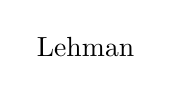
\begin{tikzpicture}
  \node at(0,0) {Lehman};
\end{tikzpicture}

\begin{tikzpicture}
\begin{axis}[
    no marks,
    date coordinates in=x,
    xticklabel=\year,
    yticklabel style={/pgf/number format/.cd,fixed,precision=2},
    ylabel=price,
    xlabel=time,
    every axis plot/.append style={thick, smooth}]
    \addplot table[x=time, y=value] {lehman.txt};
\end{axis}
\end{tikzpicture}

\begin{varplot}
\addplot[color=color1] table[x=time, y=value.EVT] {leh_vars.txt};
\addlegendentry{EVT}
\addplot[color=color2] table[x=time, y=value.Historical] {leh_vars.txt};
\addlegendentry{Historical}
\addplot[color=color3] table[x=time, y=value.DeltaNormal] {leh_vars.txt};
\addlegendentry{Delta-Normal}
\addplot[color=color4] table[x=time, y=value.GARCH] {leh_vars.txt};
\addlegendentry{GARCH}
\end{varplot}


\begin{tikzpicture}
  \node at(0,0) {United};
\end{tikzpicture}

\begin{tikzpicture}
\begin{axis}[
    no marks,
    date coordinates in=x,
    xticklabel=\year,
    yticklabel style={/pgf/number format/.cd,fixed,precision=2},
    ylabel=price,
    xlabel=time, 
    every axis plot/.append style={thick, smooth}]
    \addplot table[x=time, y=value] {united.txt};
\end{axis}
\end{tikzpicture}

\begin{varplot}
\addplot[color=color1] table[x=time, y=value.EVT] {united_vars.txt};
\addlegendentry{EVT}
\addplot[color=color2] table[x=time, y=value.Historical] {united_vars.txt};
\addlegendentry{Historical}
\addplot[color=color3] table[x=time, y=value.DeltaNormal] {united_vars.txt};
\addlegendentry{Delta-Normal}
\addplot[color=color4] table[x=time, y=value.GARCH] {united_vars.txt};
\addlegendentry{GARCH}
\end{varplot}

\end{document}
